\documentclass[aps, pre, preprint, groupedaddress, superscriptaddress, showkeys, showpacs] {revtex4-1}

\usepackage{amsmath}
\usepackage{mathtools}
\usepackage{amssymb}
\usepackage{amsfonts}
\usepackage{graphicx}
\usepackage{epstopdf}

% For the debug usage only
\usepackage{color}

\DeclarePairedDelimiter\bra{\langle}{\rvert}
\DeclarePairedDelimiter\ket{\lvert}{\rangle}

% Remove ugly line above reverences
\def\bibsection{\section*{\refname}} 

\begin{document}

\title{Quantum-Classical Phase Transition for Exciton-Polariton Josephson Junctions}

\author{M. E. Lebedev}
\email{m.lebedev@lmc.ifmo.ru}
\affiliation{ITMO University, St. Petersburg 197101, Russia}

\author{D. A. Dolinina}
\email{dasha.doly@gmail.com}
\affiliation{ITMO University, St. Petersburg 197101, Russia}


\author{A. P. Alodjants}
\email{alexander\_ap@list.ru}
\affiliation{ITMO University, St. Petersburg 197101, Russia}

\date{\today}

\begin{abstract}
We consider the quantum phase problem for low branch exciton polariton condensate Josephson junctions operating at finite temperatures and polariton lifetime. The process of quantum tunneling we characterized by thermon lifetime. We have shown that classical (thermal) activation and quantum tunneling for the phase  represent two regimes depending on polariton condensate parameters and distance between the junctions. The transition between this two regimes   exhibits universal features of first or second order phase transition depending on the potential shape for the relative phase. Notably, scale of the crytical temperature  characterized by polariton interaction strength only. We have shown that polariton condensate junction device runs in classical way for ten of Kelvins temperatures and typical polariton densities used in current experiments with narrow band semiconductor samples. Purely  quantum phase regime can be obtained even in the presence of dissipation at one or two order lower temperatures and relatively short operating time scales (few of picoseconds), and   opens kindly new possibilities for exciton polariton BEC applications in scalable quantum computing and quantum metrology.   
\end{abstract}

\pacs{\dots}
\keywords{\dots}

\maketitle

\newcommand{\sn}{\textrm{sn}}
\newcommand{\cn}{\textrm{cn}}
\newcommand{\dn}{\textrm{dn}}
\newcommand{\sd}{\textrm{sd}}
\newcommand{\cd}{\textrm{cd}}
\newcommand{\nd}{\textrm{nd}}
\newcommand{\am}{\textrm{am}}

% For the debug usage only
\newcommand{\red}{\color{red}}

\section{Introduction \label{sec:introduction}}

For last decade investigations of exciton polariton Bose-Einstein condensates (BEC) in various type of semiconductor microstructures represent one of mainstreams of current photonic and semiconductor technologies, see e.g. \cite{Sanvitto,Guillet}.
The microcavity exciton polaritons are bosonic quasiparticles representing  admixtures of the quantized cavity mode and quantum wells excitons.
Practically, semiconductor microcavities are promising for various optoelectronic applications where quantum  matter-field interface plays crucial role.
In particular, demonstrations of polariton laser with electrical pump \cite{Bhattacharya,Schneider}, amplifiers \cite{Niemietz}, switches \cite{Amo_2010}, transistors \cite{Ballarini}, polariton circuits and optical logic elements \cite{Sturm,Liew}.
Although exciton polariton condensates exhibits Bose-Einstein statistics under the phase transition condition and macroscopic occupation of the ground state at certain pumping rate that is less than for convenient lasers, they are not in true thermodynamic equilibrium state \cite{Byrnes_2014,Sun}.
  
Non-equilibrium, or, thermodynamically quasi-equilibrium features of exciton polariton condensates play certain role in various manifestations of their collective (many body) quantum states such as superfluidity \cite{Carusotto_2013,Amo_2009}, quantized vortices \cite{Lagoudakis_2008,Lagoudakis_2009}, soliton formation \cite{Sich}, Josephson oscillations and macroscopic self-trapping \cite{Abbarchi,Lagoudakis_2010}.
Since exciton polariton BEC's in present experiments examined at high enough (up to the room) temperatures the quantum character of such a states should be examined even at equilibrium.

The problem of distinguishability of statistically classical and quantum regimes for exciton polariton condensates behavior is very actual for their practical purposes, see e.g. \cite{Dominici}; especially for their possible applications for quantum information science purposes.
Fast switching properties (the typical switching time of a few picoseconds), relatively strong nonlinear response and flexibility to external optical and/or electrical pump, spin degrees of freedom made microcavity polaritons potentially very promising for quantum computation and quantum information processing objectives, see, e.g. \cite{Demirchyan,Pagel,Kyriienko,Solnyshkov_2015, Dominici}.
Especially it is important to stress quantum annealing problem \cite{Yan} that is very actual now and where collective (bosonic) character of polariton BEC could be used.
In particular, as it is shown recently in \cite{Lewenstein} global minimum of energy landscape can be reached at finite temperatures via a combination of thermal annealing and quantum tunneling. 

Another promising area of potential applications of quantum exciton polariton states is connected with quantum metrology purposes for which designing of quantum interferometers and gyroscopes possessing high precision measurements with quantum phase states is utilized, cf. \cite{Pezze, Gulevich}.
  
In the paper we consider generic problem  of quantum-classical phase transition (see e.g.\cite{Chudnovsky_1997}) with exciton polariton condensates occurring in semiconductor microcavity in the presence of Josephson effect, cf. \cite{Aleiner, Shelykh_2008, Borgh_2010}.
In general this problem relates to dissipative tunneling problem or, tunneling at finite (non-zero) temperatures models, cf. \cite{Caldeira, Larkin, Riseborough}.
Traditionally  seminal studies on this topic are based on consideration of superconductor devices \cite{Ankerhold} where macroscopic tunneling plays essential role.
In particular, it is worth to mention here Schr\"odinger cat state formation \cite{Leggett} and design of quantum gates for quantum computing with superconductor qubits where macroscopic quantum coherent phase properties are used \cite{Makhlin}.
Latterly the problem of quantum tunneling and quantum-classical phase transition problem have been applied to other two-level (spin) systems, like atomic BEC's \cite{Zhang}, and small ferromagnetic particles, \cite{Owerre}.
Strictly speaking main discussion is focused on investigation of quantum-classical escape rate transition that takes place in the presence of potential barrier at finite temperatures.
  
In the paper we propose \textit{extended model} for exciton polariton Josephson junctions that relates to so-called non-standard Bose-Hubbard models (see \cite{Dutta} and references therein) when energy of polariton-polariton scattering contributes into the tunneling parameter, cf. \cite{Aleiner, Shelykh_2008, Borgh_2010, Solnyshkov_2008, Sarchi}.
In particularly, we pay our attention to temperature dependent quantum critical phenomena occurring in the presence of macroscopic tunneling.
We aimed at elucidation of necessary criteria to obtain quantum phase regimes with trapped exciton polaritons suitable for creation of exciton polariton qubit gates.

This paper is arranged as follows.
In Sec. \ref{sec:model} we explain in details our model to realize Josephson junction with exciton polariton condensates.
The extended tight-binding model will be established in this case.
In Sec. \ref{sec:quantum_phase} we {\red \dots }.
In the conclusion, we summarize the results obtained.

\section{THE MODEL OD EXCITON POLARITON JOSEPHSON JUNCTION \label{sec:model}}

We start by describing the problem of equilibrium exciton polariton condensate trapping in symmetric one dimensional double-well potential $U(x) = h ((x/x_0)^2 - 1)^2$; $2x_0$ defines distance between potential minima, $h$ depth of the potential.
% 
%\begin{figure}[ht]
%\center{\includegraphics[width=0.5\linewidth]{pic/potential_sym_asym.png}}
%\caption{
%Confined double-well potential for exciton polariton coupled condensate channels with symmetric $(\Phi_+(x))$ and asymmetric $(\Phi_-(x))$ wavefunctions obtained numerically by solving stationary GPE (\ref{eq:stationary}).
%The dimensionless parameters for the calculations are: $h = 10$, $x_0 = 1$, $\mu_+ = 5.7355$, $\mu_- = 6.5653$.
%\label{pic:potential_sym_asym}

%\end{figure}
%
The Hamiltonian for the system of weakly interacting exciton polaritons in an external $U(x)$ can be written in the second quantized form as:
%
\begin{equation}
\hat{H} = \int \Big\{ -\dfrac{\hbar^2}{2m} \hat{\psi}^\dag \dfrac{d^2 \hat{\psi}}{dx^2} + \hat{\psi}^\dag \hat{\psi} U(x) + \dfrac{g}{2} \hat{\psi}^{\dag 2} \hat{\psi}^2  \Big\} dx,
\label{eq:gpe_hamiltonian}
\end{equation}
%
where $\hat{\psi} \equiv \hat{\psi}(x, t)$ is a polariton field operator that annihilate a particle at the position $x$ and time $t$, $g$ is two-body (polariton-polariton) scattering length.
In the paper we use so-called two-mode representation of $\hat{\psi}$ - operator supposing
%
\begin{equation}
\hat{\psi} = \hat{\psi}_1(t) \Phi_1(x) + \hat{\psi}_2(t) \Phi_2(x),
\label{eq:two_modes}
\end{equation}
%
where $\hat{\psi}_{1,2}$ are time dependent operators characterizing condensate at the left and at the right wells respectively; $\Phi_{1,2}(x)$ are condensate wavefunctions which are responsible for it spatial distribution.
It's instructive to recast $\Phi_{1,2}(x)$ as
%
\begin{equation}
\Phi_{1,2} = \dfrac{\Phi_+ \pm \Phi_-}{\sqrt{2}}
\label{eq:basic_modes}
\end{equation}
%
where $\Phi_{\pm}(x) = \pm \Phi_{\pm}(-x)$ are symmetric ($\Phi_+$) and antisymmetric ($\Phi_-$) real wavefunctions obeying stationary Gross-Pitaevskii equations $\mu_{\pm} \Phi_{\pm} = -\dfrac{\hbar^2}{2m} \dfrac{d^2 \Phi_{\pm}}{dx^2} + U(x) \Phi_{\pm} + g \Phi_{\pm}^3$.
%
%\begin{equation}
%\mu_{\pm} \Phi_{\pm} = -\dfrac{\hbar^2}{2m} \dfrac{d^2 \Phi_{\pm}}{dx^2} + U(x) \Phi_{\pm} + g \Phi_{\pm}^3.
%\label{eq:stationary}
%\end{equation}
%
and normalization condition $\int \Phi_{\pm}^2 dx = 1$.
Here $\mu_{\pm}$ are chemical potentials.
As a result an operator $\hat{\psi_1}^\dag\hat{\psi_1} + \hat{\psi_2}^\dag\hat{\psi_2} = N$ characterizes total number of particles (here and thereafter we omit ``hat'' design for simplicity).
Substituting (\ref{eq:basic_modes}), (\ref{eq:two_modes}) into (\ref{eq:gpe_hamiltonian}) we arrive to
% 
\begin{equation}
\begin{array}{lcl}
\hat{H} & = & \dfrac{A}{2} (\hat{\psi}_1^{\dag 2} \hat{\psi}_1^2 + \hat{\psi}_2^{\dag 2} \hat{\psi}_2^2) - \dfrac{G}{2} (\hat{\psi}_1^\dag \hat{\psi}_2 + \hat{\psi}_1 \hat{\psi}_2^\dag) \\ [8pt]
& & -\dfrac{\Gamma}{2} (\hat{\psi}_1^{\dag 2} \hat{\psi}_1 \hat{\psi}_2 + \hat{\psi}_1^\dag \hat{\psi}_1^2 \hat{\psi}_2^\dag + \hat{\psi}_1^\dag \hat{\psi}_2^\dag \hat{\psi}_2^2 + \hat{\psi}_1 \hat{\psi}_2^{\dag 2} \hat{\psi}_2) \\ [8pt]
& & +\dfrac{C}{2} (\hat{\psi}_1^{\dag 2} \hat{\psi}_2^2 + 4 \hat{\psi}_1^\dag \hat{\psi}_1 \hat{\psi}_2^\dag \hat{\psi}_2 + \hat{\psi}_1^2 \hat{\psi}_2^{\dag 2}),
\end{array}
\label{eq:hamiltonian}
\end{equation}
%
where we made some denotations $\gamma_{ij} = g \int \Phi_i^2 \Phi_j^2 dx, i,j \in \{+,-\}$;
$A = \frac{1}{4} (\gamma_{++} + \gamma_{--} + 6 \gamma_{+-})$; $\Gamma = \frac{1}{2} (\gamma_{++} - \gamma_{--})$; $C = \frac{1}{4} (\gamma_{++} + \gamma_{--} - 2\gamma_{+-})$; $G = \mu_- - \mu_+ - 2\Gamma$.

Hamiltonian (\ref{eq:hamiltonian}) represents extended model for internal Josephson junction effect with exciton polariton BEC trapped in double-well potential.
The ``additional'' terms with $\Gamma$ and $C$ in (\ref{eq:hamiltonian}) characterize density induced and pair tunneling, respectively.
Generally, our model implies existence of quantum tunneling of the particles between wells with effective (nonlinear) tunneling rate $G_{eff} = \dfrac{1}{2}(G+\Gamma N - C\hat{\psi}_1^\dag\hat{\psi}_2)$.
The contribution from relevant coefficients on can be estimated from variational ansatz
%
\begin{equation}
\Phi_{\pm} = A_{\pm} \Big[ \exp \Big( -\dfrac{(x - x_0)^2}{2 a^2} \Big) \pm \exp \Big( -\dfrac{(x + x_0)^2}{2 a^2} \Big) \Big]
\label{eq:two_modes_eq}
\end{equation}
%
where $a$ is width of condensate wavefunctions at each wells (we suppose them equal to each other), defined from normalization conditions.
In Fig. \ref{pic:gamma_pm_vs_g} the behavior of normalized coefficients $\dfrac{\gamma_{ij}}{g}$ $i,j \in \{+,-\}$ as a function of half of intra-well distance $x_0$ is shown.
It is important that at differences between them rapidly vanishes with increasing of distance $x_0$.
We can suppose $\Gamma = C = 0$ for $x_0 >> a$.
This limit exactly corresponds to familiar problem of two weakly linked condensates at zero temperature, see e.g. \cite{Aleiner, Shelykh_2008, Borgh_2010, Raghavan}.
%
\begin{figure}[ht]
\center{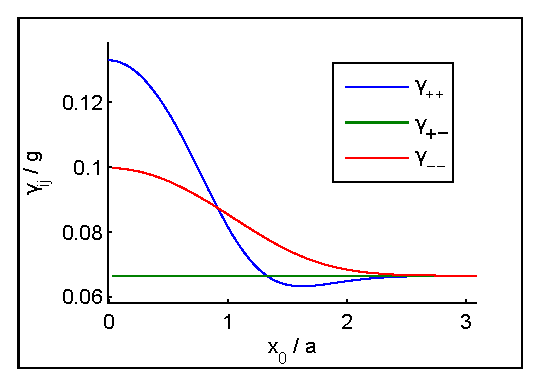
\includegraphics[width=0.5\linewidth]{pic/ypm_x0.eps}}
\caption{Dependence of $\gamma_{ij} / g$ on $x_0 / a$ \label{pic:gamma_pm_vs_g}}
\end{figure}
%

\section{The Quantum Phase \label{sec:quantum_phase}}

To elucidate purely quantum phase features of our extended Josephson model it is fruitful to recast Hamiltonian (\ref{eq:hamiltonian}) through the pseudo-spin operators defined as
% 
\begin{subequations}
\begin{align}
\hat{S}_x = & \dfrac{1}{2} (\hat{\psi}_1^\dag \hat{\psi}_2 + \hat{\psi}_1 \hat{\psi}_2^\dag) = s \cos{\phi} - \sin{\phi} \dfrac{d}{d \phi}, \\
\quad \hat{S}_y = & \dfrac{i}{2} (\hat{\psi}_1^\dag \hat{\psi}_2 - \hat{\psi}_1 \hat{\psi}_2^\dag) = s \sin{\phi} + \cos{\phi} \dfrac{d}{d \phi}, \\
\hat{S}_z = & \dfrac{1}{2} (\hat{\psi}_2^\dag \hat{\psi}_2 + \hat{\psi}_1^\dag \hat{\psi}_1) = -i\dfrac{d}{d \phi},
\end{align}
\label{eq:pseudo_spin}
\end{subequations}
%
where  $\phi$ is the phase variable.
The operators determined in Eq. (\ref{eq:pseudo_spin}) obey familiar $SU(2)$ algebra commutation relations $[S_i, S_j] = i\epsilon_{ijk}S_k,  i,j,k=x,y,z$.

After straitforward calculations from (\ref{eq:hamiltonian}) one can obtain
%
\begin{equation}
\begin{array}{lcl}
H & = & -(\alpha - \beta \sin^2 \phi) \dfrac{d^2}{d \phi^2} - (\beta(s-\dfrac{1}{2})\sin{2\phi} - B\sin{\phi}) \dfrac{d}{d \phi} \\
&& - Bs \cos \phi - \beta s^2 \sin^2 \phi - \beta s \cos^2 \phi.
\end{array}
\label{eq:hamiltinian_s}
\end{equation}
%
where $\alpha = A - C = 2\gamma_{\pm} > 0$, $\beta = 2C > 0$ and $B = \Gamma N + G > 0$.
Below we chose $x_0$ obeying to condition $\gamma_{++} \simeq \gamma_{--} = \gamma$ supposing $\Gamma = 0$ for simplicity, see Fig. \ref{pic:gamma_pm_vs_g}. We also assume macroscopically large particle number, that is $s = \dfrac{N}{2} >> 1$ is C - number. Using (\ref{eq:hamiltinian_s})  for Schrodinger equation we obtain   
%
\begin{equation}
\begin{array}{l}
(\alpha - \beta \sin^2 \phi) \dfrac{d^2 \Phi}{d \phi^2} + (\beta s\sin{2\phi}-B\sin{\phi})) \dfrac{d \Phi}{d \phi} \\
+ s(B \cos \phi + \beta s \sin^2 \phi) = 0.
\end{array}
\label{eq:schrodinger}
\end{equation}
%
where $\Phi \equiv \Phi(\phi)$ is unknown $2\pi$-periodic wavefunction that characterizes quantum phase properties, cf. \cite{Anglin}.
%ng that Eqs. (\ref{eq:hamiltinian_s}), (\ref{eq:schrodinger}) can be obtained by applying so-called phase-state representation, {\red cf. [  ]}.
%
%\begin{equation}
%\ket{\psi} = \dfrac{1}{2 \pi} \int_{-\infty}^{+\infty} d \phi \Phi(\phi) \ket{\phi}
%\end{equation}
%
%where
%
%\begin{equation}
%\ket{\phi} = \dfrac{1}{\sqrt{N!}} \Big[ e^{i\phi/2} \psi_1^\dagger + e^{-i \phi/2} \psi_2^\dag \Big]^N \ket{0}_1\ket{0}
%\end{equation}
%
%is macroscopic coherent spin-state (macroscopic qubit state) that plays important role in current quantum information protocols operating with $N$-particle condensates, cf. \cite{Byrnes_2012}.
It is possible to eliminate the term with first derivative in Eq. (\ref{eq:schrodinger}) applying the transformation
%
\begin{equation}
\Phi(\phi) = \Psi(z) \exp \Big( s \ln \dn{z} - \dfrac{\Lambda s}{2 \sqrt{\lambda (1 - \lambda)}} \arctan \Big( \sqrt{\dfrac{\lambda}{1 - \lambda}} \cn{z} \Big) \Big)
\label{eq:transformation_of_phi}
\end{equation}
%
where $z = \int \limits_0^\phi \dfrac{d \xi}{\sqrt{1 - \lambda \sin^2 \xi}} = F(\phi, \lambda)$ is new phase variable; $F(\phi, \lambda)$ is incomplete elliptic integral of the first kind.
In (\ref{eq:transformation_of_phi}) we have introduced dimension-less parameters $\Lambda = \dfrac{G}{\alpha s}$, $\lambda = \dfrac{\beta}{\alpha}$ playing crucial role in our model.
Inserting (\ref{eq:transformation_of_phi}) into (\ref{eq:schrodinger}) we arrive to Schr\"odinger-like equation
% 
\begin{equation}
\alpha \frac{d^2\Psi}{dz^2} + (E - V(z))\Psi = 0
\label{eq:schrodinger_usual}
\end{equation}
%
for quantum particle with the ``mass''  $m = \dfrac{\hbar^2}{2 \alpha}$ and energy $E$, that moves in the potential $V(z) = \alpha s^2 V_0(z)$ with
%
\begin{equation}
V_0(z) = \frac{ (\frac{1}{4} \Lambda^2 - \lambda (1 - \lambda)) \sn^2{z} - \Lambda \cn{z}}{\dn^2{z}}
\label{eq:potential}
\end{equation}
%

The results known for quantum phase mesoscopic Josephson junction model can be recovered from (\ref{eq:hamiltonian}), (\ref{eq:potential}) at $\lambda = 0$.
The dependence of the $\lambda$ parameter on normalized half of intra-well distance $\dfrac{x_0}{a}$ can be estimated from (\ref{eq:two_modes_eq}) and reads as $\lambda = 0.5 \Big( \exp \Big[ \dfrac{2 x_0^2}{a^2} \Big] - 1 \Big)^{-1}$.
The limit $\lambda = 0$ corresponds to  infinitely large intra-well distances with $x_0 \to \infty$.
On the other hand, parameter grows rapidly at $\dfrac{x_0}{a} \ll 1$.
Obviously, in this limit our Josephson junction model inherent based on relatively weak coupling between wells breaks down.
Below we examine case of $0 < \lambda < 1$ that could be obtained at moderate values $\dfrac{x_0}{a}$ of such as $\dfrac{x_0}{a} \geq 0.45$. 

Analysis of the quantum phase could be examined in three domains of vital parameter $\Lambda$, cf. \cite{Anglin}.
The dependences of trapping potential $V_0(x)$ are shown in Fig. \ref{phase_potential}.
The period of the functions is determined as $4K(\lambda)$.
%
\begin{figure}[ht]
\begin{center}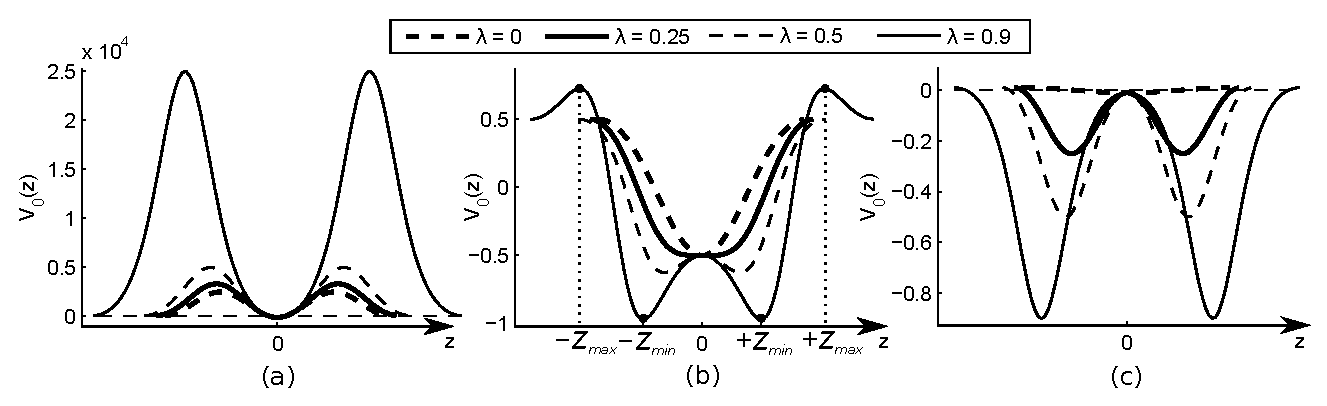
\includegraphics[width=1\linewidth]{pic/potentials.eps}
\end{center}
\caption{
Effective potential $V_0(z)$ for (a) $\Lambda = 100$, (b) $\Lambda = 0.5$ , and (c) $\Lambda = 0.01$ as a function of  elliptic integral phase coordinate $z$.
Points $\pm z_{min}$ and $\pm z_{max}$ in (b) corresponds to global minima and maxima of the potential, correspondingly, occurring with periodicity $4K(\lambda)$. \label{phase_potential}}
\end{figure}
%

\textit{Rabi regime} $\Lambda \gg 1$. In this limit the trapping potential reads $V_R(z) = \dfrac{1}{4} \Lambda^2 \sd^2{z}$.
Physically, for any value of $\lambda$ -- parameter taken from the domain $\lambda <1$ we can obtain phase (Rabi) oscillations.
In particular, small amplitude oscillations which are inherent to familiar Rabi regime can be achieved for negligable $\lambda$ --- see Fig. \ref{phase_potential}a and cf. \cite{Anglin}.

\textit{Josephson regime} $1/N^2\ll\Lambda <1$.
This regime represents intermediate case between Rabi and Fock limits --- see Fig. \ref{phase_potential}b.
The behavior of the phase depends on the ratio between parameters $\Lambda$ and $\lambda$.
If $\Lambda \ge 2\lambda$ the $V_0(z)$ posses only one minima at $z = 0$ and $V(0) = -\Lambda$. 
%Frequency of small amplitude ($z \ll 1$) oscillations %can be obtained from (\ref{eq:potential}) and looks like { \red $\omega_{0, quantum} = \frac{2 \alpha s}{\hbar} \sqrt{\frac{1}{4} \Lambda^2 - \frac{\Lambda}{2} (2\lambda - 1) - \lambda(1 - \lambda)}$ }.

In the other limit, for $\Lambda < 2 \lambda$, quantum particle is trapped at two minima of $V_0(z)$ that correspond to $W$ -- like potential with coordinates $\cn{z_{min}} = \frac{\Lambda}{2 \lambda}$ and appearing for both of Josephson and Fock regimes, cf. Fig. \ref{phase_potential}b,c.  
The depth of the potential minima depends on the $\lambda$ parameter.
It is interesting to note that for $\Lambda > 2(1 - \lambda)$ potential $V_0(z)$ presumes local minimum at $\pm 2 K(\lambda)$ that is marked by red point $C$ in Fig. 3b.

\textit{Fock regime} $\Lambda \ll 1/N^2$.
In purely quantum limit the two mode system approaches by the state $\ket{\psi} \propto (\psi_1^\dag)^s (\psi_1^\dag)^s \ket{0}_1 \ket{0}_2$ with the phase wavefunction $\Phi(\phi) \to (2\pi)^{-1/2}$.
In this regime, when inequality $\Lambda \ll \lambda < 1$ is holds, Eq.(\ref{eq:schrodinger_usual}) transforms into Mathieu equation that implies spectrum consisting from all Mathieu functions.
% $ce_0(z, q)$, $ce_1(z, q)$, $se_1(z, q)$, \dots, which are $2\pi$-periodic, and corresponding eigenvalues $a$ can be found using series expansions in powers of $q$.
%from (\ref{eq:potential}) one can obtain
%
%{\red

%
%\begin{equation}
%V_F(z) \simeq -\lambda (1 - \lambda) \sin^2{z},
%\end{equation}
%
%and our 
%transforms into Mathieu equation;
%
%\begin{equation}
%\frac{d^2 \Psi}{d z^2} + (a - 2q  \cos{2z}) \Psi = 0.
%\end{equation}
%
%where $a = E / \alpha + s^2 \lambda(1 - \lambda) / 2$, $q = s^2 \lambda (1 - \lambda)/ 4$.
%We recall our boundary condition: $\Psi(z + 2\pi) = \Psi(z)$.



%In another limit $\lambda \ll \Lambda$ 
%that might  be studied within Fock regime is relevant to condition . In this case from (\ref{eq:potential}) 
%we have $V_0(z) \simeq -\Lambda \cos{z}$.
%In fact, this limit that deals with negligible $\lambda$ reproduces results for convenient quantum phase model \cite{Anglin}.


\section{Quantum-classical phase transitions \label{sec:quantum_classical}}

Strictly speaking, results established in previous section are completely valid at zero temperature. However, in current experiments with exciton polaritons  the condensate is observed at finite and high enough temperatures.
In this section we find answer to vital question: when quantum approach to the phase problem for Josephson junction with coupled exciton polariton condensates is valid?

To give an answer to this question we consider the effective $W$ -- like potential represented in Fig. \ref{phase_potential}b,c inherent to  Josephson (or, Fock) regimes, respectively.
To be more specific we examine thermodynamically equilibrium system at finite temperature $T$.  Transition between two stable states (say, between points $z_{1,2}$ in Fig. \ref{phase_potential}b) can happen  either through the quantum tunneling or, in classical way, due to the thermal activation. 
Obviously, at high temperatures such as $k_{B}T\ge\Delta V$ ($\Delta V$ is height of the barrier between two states with minimum of potential energy) the particle undergoes hopping over the barrier governed by familiar thermoactivation (Arrhenius) escape rate $\Gamma \sim e^{-\Delta V /k_{B}T}$, cf. \cite{Larkin}.
On the other hand, in the ``low temperature'' limit $k_{B}T\ll\Delta V$ particle undergoes quantum tunneling through the barrier with vanishing rate.
%with the rate $\Gamma \sim e^{-B/\hbar}$, where $B$ is the instanton action.
%Now we elucidate conditions for their realization for exciton polariton Josephson junction problem. 

Our description for exciton polariton Josephson junction problem is based on imaginary time path integral approach, cf. \cite{Ankerhold}.
The imaginary-time action obtained within WKB method approaches as $S(E) = \oint (\tfrac{1}{2} m \dot{z}^2 + V(z)) d \tau$.
%
%\begin{equation}
%S(E) = \oint (\tfrac{1}{2} m \dot{z}^2 + V(z)) d \tau.
%\label{eq:thermon_action_1}
%\end{equation}
%
The decay rate $\Gamma \sim e^{-S_{min}/\hbar}$ according our approach can be expressed through the minimal value $S_{min}$ of the action.
The trajectories which are minimize the action $S_T$ satisfy to classical equation of motion $m \ddot{z} = \frac{d V}{dz}$ written for the thermon that  oscillates inside the inverted potential $-V(z)$. 
%
%\begin{equation}
%m \ddot{z} = \frac{d V}{dz}.
%\label{eq:thermon}
%\end{equation}
%
Periodic solutions of this equation satisfy the relation
%
\begin{equation}
\tfrac{1}{2} m \dot{z}^2 = V(z) - E(\tau_p),
\label{eq:total_energy}
\end{equation}
%
where $\tau_p = \hbar / k_B T$ is a thermon period corresponding to the energy $E(\tau_p)$;
%
\begin{equation}
\tau_p(E) = \sqrt{2 m} \int_{z_1(E)}^{z_2(E)} \frac{dz}{\sqrt{V(z) - E}}.
\label{eq:thermon_period}
\end{equation}
%
In (\ref{eq:thermon_period}) the $z_{1,2}(E)$ are turning points, cf. Fig. \ref{phase_potential}b.
The Eqs.(\ref{eq:total_energy}),(\ref{eq:thermon_period}) taken at energy $E = 0$ and temperature $T = 0$ characterize instanton solution.
Combining  equation for $S(E)$ 
%(\ref{eq:thermon_action_1}) 
with (\ref{eq:total_energy}) we obtain  
%
\begin{equation}
S_T = 2 \sqrt{2 m} \int_{z_1(E)}^{z_2(E)} \sqrt{V(z) - E} ~dz + E \tau_p (E).
\label{eq:thermon_action_2}
\end{equation}
%

To determine thermodynamic properties of the system it is necessary to know small amplitude oscillations  at the bottom, $z=0$, of inverted potential $-V(z)$.
The action in this case reads: 
%
\begin{equation}
S_0 = \Delta V \tau_p (E).
\label{eq:thermal_action}
\end{equation}
%

Expansion of the potential $V(z)$ excluding constant value $V(0)$ gives:
%
\begin{equation}
\begin{array}{lcl}
V(z) & = & \alpha s^2 \Big[ \left( \frac{1}{4} \Lambda^2  - \frac{2\lambda - 1}{2} \Lambda - \lambda (1 - \lambda) \right) z^2 \\
&& + \left( \frac{2\lambda - 1}{12} \Lambda^2 - \frac{16\lambda^2 - 16\lambda + 1}{24} \Lambda - \frac{\lambda (1 - \lambda) (2\lambda - 1)}{3} \right) z^4 + o(z^4) \Big].
\end{array}
\label{eq:potential_teylor}
\end{equation}
%
In particularly, if the inverted potential $-V(z)$ has the form $z^2 - z^4$ the second order phase transition occurs.
If $-V(z)$ behaves as $z^2 + z^4$ first order phase transition take place.
Phase boundary between 1st and 2nd order phase transitions is determined by the relation
%
\begin{equation}
\Lambda = \frac{1 - 16\lambda + 16\lambda^2 + \sqrt{1 + 32\lambda - 32\lambda^2}}{4(2\lambda - 1)}.
\label{eq:order_border}
\end{equation}
%
We summarize our results in the Fig. \ref{pic:phase_boundary_combined}.  First order phase transition occurs in the shaded region for two type of potentials only. 
%
\begin{figure}[ht]
\center{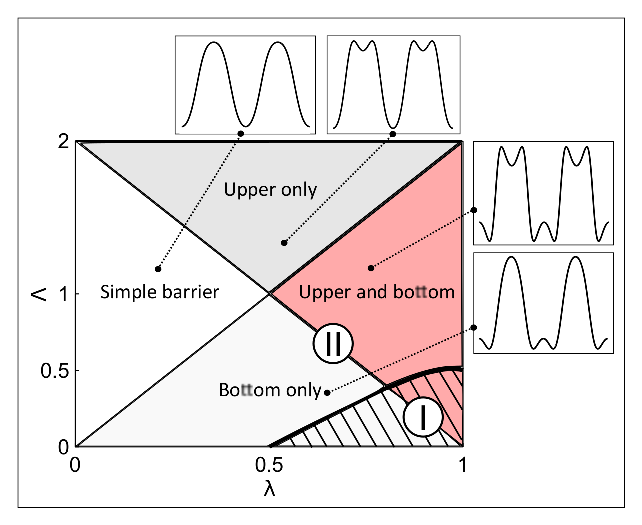
\includegraphics[width=0.5\linewidth]{pic/phase_transition_diagram_combined.eps}}
\caption{Diagram of the phase boundary for  first- and second-order  phase transitions in $\Lambda$,$\lambda$-parameter plane \label{pic:phase_boundary_combined}}
\end{figure}
%

The crossover temperature of second-order phase transition $T_{c}^{(2)} = \hbar \omega_0/ 2 \pi k_B$ is 
%
\begin{equation}
T_{c}^{(2)} = T_{0} \sqrt{\lambda (1 - \lambda) + (2 \lambda - 1) \tfrac{\Lambda}{2} - \tfrac{1}{4} \Lambda^2},
\label{eq:second_order}
\end{equation}
%
where  $\omega_0 = \frac{2 \alpha s}{\hbar} \sqrt{\lambda (1 - \lambda) + \tfrac{1}{2} (2 \lambda - 1) \Lambda - \tfrac{1}{4} \Lambda^2}$ is small oscillation frequency of thermon near the bottom of inverted potential, $T_{0}=\alpha N / 2\pi k_B$ is critical temperature $T_{c}^{(2)}=T_{0}$ taken at $\Lambda=2\lambda-1$.
The characteristic temperature $T_{0}$ discussed above implies important time scale $\tau_0=2\pi\hbar/ \alpha N$ that can be understood as thermon ``lifetime''.
From (\ref{eq:second_order}) follows that, for $\Lambda \ge 2\lambda$ there is no barrier at $z = 0$.

%
\begin{figure}[ht]
\begin{minipage}[h]{0.49\linewidth}
\center{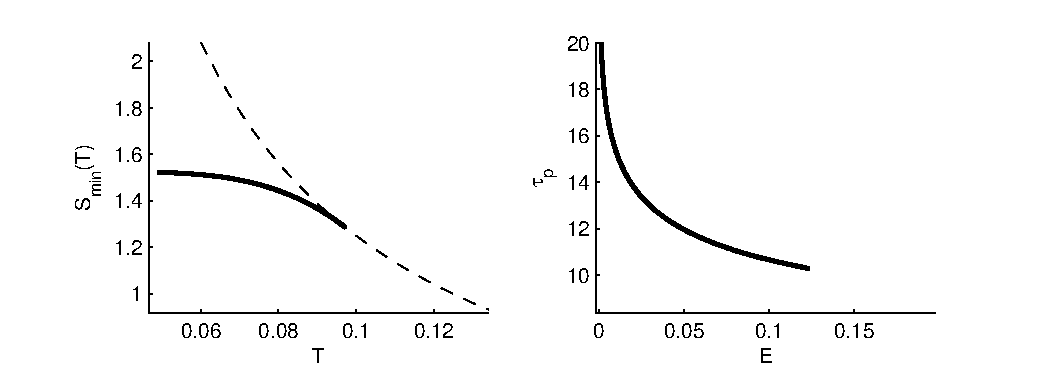
\includegraphics[width=1\linewidth]{pic/action_period_2nd_order_transition.eps} \\ (a)}
\end{minipage}
\hfill
\begin{minipage}[h]{0.49\linewidth}
\center{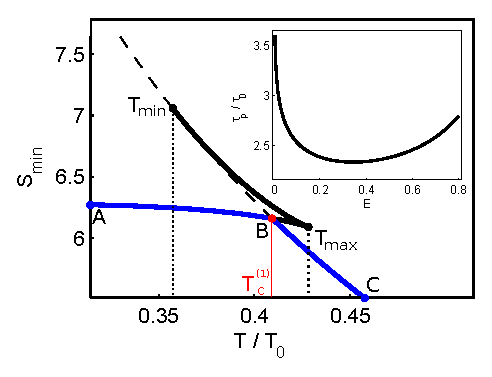
\includegraphics[width=1\linewidth]{pic/action_period_1st_order_transition.eps} \\ (b)}
\end{minipage}
\caption{Dependences of  minimal action $S_{min}$ (ABC-curve) taken in $s\hbar$ units as a function of reduced temperature $ T/T_{0}$ for (a) 2nd-order transition, $\lambda = 0.9$, $\Lambda = 0.1$; and, (b) 1st-order transition, $\lambda = 0.5$, $\Lambda = 0.5$; the solid (bold) line corresponds to the thermon action, $S_T$; the dashed line corresponds to the thermodynamic action, $S_0 = \hbar \Delta V / k_B T$, $S_{min} = \min \{S_0, S_T\}$. The inset shows dependences of  dimensionless $\tau_p / \tau_0$ versus energy $E$ given in  $\alpha s^2$ units. 
\label{pic:action_period}}
\end{figure}
%

The Fig. \ref{pic:action_period}a displays second-order phase transition from quantum (solid bold line of $S_T$) to thermal (classical) regimes --- dashed bold line of $S_0$.
The crossover occurs at the critical point $T_{c}^{(2)}$ where $S_T = S_0$ and {$E = E_0$}.
The inset demonstrate monotonic dependence of thermon period $\tau_p$ on energy $E$ that is inherent to second-order phase transition.
Closest to the critical point with energy $E=E_0$ thermon undergoes small amplitude oscillations.  
  
In Fig. \ref{pic:action_period}b we represent results exhibiting first-order phase transition.
It is clearly seen that the first derivative of $S_{min}$ is discontinuous in this case and the dependence of thermon period $\tau_p$ on energy $E$ is non-monotonic (see inset in Fig. \ref{pic:action_period}b).
The critical temperature $T_{c}^{(1)}$ belongs to the temperature domain $T_{min} < T_{c}^{(1)} < T_{max}$ and can be find out numerically by solving Eqs.(\ref{eq:thermon_period}) - (\ref{eq:thermal_action}) under the condition $S_T = S_0$.
 
Analytically critical temperature $T_{c}^{(1)}$ meight be estimated from $T_{c}^{(1)} = \Delta V / B$, where $B$ is a instanton action that can be represented as $B = S(E_{min})$.
After some straightforward calculations for $B$ we obtain
%
\begin{equation}
\begin{array}{c}
B = S(E_{min}) = 2 s \hbar \left[ \ln \frac{2 \sqrt{\lambda} + \sqrt{4 \lambda^2 - \Lambda^2}}{2 \sqrt{\lambda} - \sqrt{4 \lambda^2 - \Lambda^2}} - \frac{\Lambda}{\sqrt{\lambda (1 - \lambda)}} \arctan \left( \frac{\sqrt{(1 - \lambda) (4 \lambda^2 - \Lambda^2)}}{\Lambda} \right) \right].
\end{array}
\label{eq:B_action}
\end{equation}
%

In current experiments it is much more easier to manipulate be the density of exciton polaritons instead of their temperature due to some  non-equilibrium processes occurring in real microcavity samples, see e.g. \cite{Sanvitto,Guillet}.
For instance, the density of polariton gas can be manipulated by using the optical pump.
In Fig. \ref{pic:temperatures} we plot numerically calculated critical temperature of 1st and 2nd order phase transitions against $\Lambda$-parameter for experimentally accessible semiconductor Josephson junction samples.
The solid (green) line corresponds to analytical solution obtained with  Eq. (\ref{eq:B_action}).
Since the $\Lambda$-parameter is inversionally proportional to the density of exciton polariton gas (so-called blue shift) Fig. \ref{pic:temperatures} establishes important correspondence between critical temperatures discussed in the paper and relevant exciton polariton densities.
%
\begin{figure}[ht]
\center{\includegraphics[width=0.5\linewidth]{pic/phase_transition_temperatures.eps}}
\caption
{Dependence of dimensionless critical temperature $T_{c}/T_{0}$ as a function of parameter $\Lambda$. Solid (green) line corresponds to analytical solution for  $T_{c}^{(1)}$.     
\label{pic:temperatures}}
\end{figure}
%

Now let us briefly discuss decay of the upper state that is relevant to the point C in ..... and exist for $\Lambda > 2(1 - \lambda)$.
Potential presumes local minima at $\pm 2K(\lambda)$ and local maxima at $z_{max} = \pm \cn^{-1} \left( -\frac{2(1 - \lambda)}{\Lambda} \right)$.
Equation for the thermon yields 
%small ocsillation frequency near the bottom $z_{max}$ of the inverted potential $\omega_0 = \frac{\alpha s}{\hbar} \sqrt{\frac{\Lambda^2}{1 - \lambda} - 4(1 - \lambda)}$.
crossover temperature of second-order phase transition $T_{c}^{(2)} = (T_{0}/ 2) \sqrt{\frac{\Lambda^2}{1 - \lambda} - 4(1 - \lambda)}$, cf.... 
%
%\begin{equation}
%T_{c}^{(2)} = (T_{0}/ 2) %\sqrt{\frac{\Lambda^2}{1 - \lambda} - 4(1 - \lambda)}.
%\label{eq:second_order_2}
%\end{equation}
%
By expanding the potential $V(z)$ near the vicinity of $z_{max}$ it is possible to show that only second-order phase transition appear for this case.

%With the aim of analytical determining of the phase transition order let's write the Taylor series for $V(z)$ near the vicinity of $z_{max}$.
%Expansion of the potential $V(z)$ excluding constant value $V(z_{max})$ gives:
%
%\begin{equation}
%V(\tilde{z}) = \alpha s^2 \Big[ -\tfrac{1}{4} \left( \tfrac{\Lambda^2}{1 - \lambda} - 4(1 - \lambda) \right) \tilde{z}^2 
%+ \tfrac{1}{2} \tfrac{\Lambda \sqrt{\Lambda^2 - 4(1 - \lambda)^2}}{\sqrt{1 - \lambda} \sqrt{\Lambda^2 + 4 \lambda (1 - \lambda}} \tilde{z}^3 + o(\tilde{z}^4) \Big],
%\label{eq:potential_teylor_2}
%\end{equation}
%
%where $\tilde{z} = z - z_{max}$.
%It follows from (\ref{eq:potential_teylor_2}) that $-V(\tilde{z})$ aways has the form $\tilde{z}^2 - \tilde{z}^3$, as $\Lambda > 0$, so in this case only second-order phase transition occurs.
% We plot typical behaviour of the $\tau(E)$, $S(T)$ and $T_{c}^{(2)}$ on Figs. \ref{pic:action_period_temperature_2}, and summarize our results on the Fig. \ref{pic:phase_boundary_combined}.
%
%\begin{figure}[ht]
%\begin{minipage}[h]{0.49\linewidth}
%\center{\includegraphics[width=\linewidth]{pic/action_period_2nd_order_transition_b2.eps} \\ (a)}
%\end{minipage}
%\hfill
%\begin{minipage}[h]{0.49\linewidth}
%\center{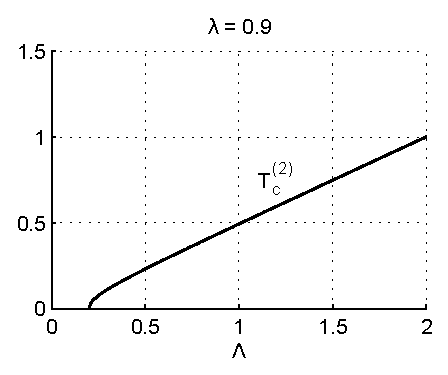
\includegraphics[width=\linewidth]{pic/phase_transition_temperatures_b2.eps} \\ (b)}
%\end{minipage}
%\caption{\dots \label{pic:action_period_temperature_2}}
%\end{figure}
%
\section{Phase transitions in the presence of dissipation 
\label{sec:non-equilibrium}}

The obtained above results for phase transitions are valid in true thermodynamically equilibrium limit. Notably  exciton polariton condensates in current experiments are out of   thermal  equilibrium, cf. [   ].  
It is obvious that for quantum tunneling effects observation  characteristic time scale $\tau_0$ should be shorter than time scales which relay to non-equilibrium processes. More precisely, in this case we require fulfillment of  inequality 
 
\begin{equation}
 \tau_{0}\ll\tau_{pol},
 \label{eq:lifetime}  
\end{equation}
where $\tau_{pol}$ characterizes  exciton polariton lifetime. However, in realistic (experimental) situation with exction polariton BEC it will be hard to obey to condition {\eqref{eq:lifetime}. In this case it is necessary to analyze dynamics of the system.      
 Below we consider the influence of the dissipation to the phase properties in adiabatic limit.

We start from mean field  equations obtained from  (\ref{eq:hamiltonian}) for  $\Gamma = 0$,  which reads as 
%
\begin{equation}
i \dot{\psi}_{1,2} = -i \kappa \psi_{1,2} +  \alpha |\psi_{1,2}|^2 \psi_{1,2} - (B/2 - \beta \psi_{1,2}^* \psi_{2,1}) \psi_{2,1}, 
\label{eq:GP}
\end{equation}
%
where we also introduced dissipation rate term with $\kappa \simeq 1/\tau_{pol}$.
By introducing new variables  $\psi_{1,2} = \Psi_{1,2} \exp(-\kappa t)$ for mean field pseudo-spin  parameters (\ref{eq:pseudo_spin}) from ({\ref{eq:GP}}) we obtain
%
%\begin{equation}
%\begin{array}{lcl}
%i \Psi_{1, t} & = & \alpha(t) |\Psi_1|^2 \Psi_1 - (B/2 - \beta(t) \Psi_1^* \Psi_2) \Psi_2; \\
%i \Psi_{2, t} & = & \alpha(t) |\Psi_2|^2 \Psi_2 - (B/2 - \beta(t) \Psi_2^* \Psi_1) \Psi_1.
%\end{array}
%\end{equation}
%
%Hamiltoninan in terms of Stocks operators (\ref{eq:pseudo_spin}):
%
%\begin{equation}
%\hat{H} = \alpha(t) \hat{S}_z^2 + \beta(t) %\hat{S}_x^2 - B \hat{S}_x.
%\end{equation}
%
%Equaitions on the mean-values of operators:
% 
\begin{equation}
\begin{array}{lcl}
\dot{S}_z & = &  2 \beta(t) S_x S_y - B S_y; \\
\dot{S}_x & = & -2 \alpha(t) S_z S_y; \\
\dot{S}_y & = & 2(\alpha(t) - \beta(t)) S_z S_z + B S_z.
\end{array}
\label{eq:pseudo-spin}
\end{equation}
%

Now set of Eqs.\ ({\ref{eq:pseudo-spin}}) looks similar to one taken for  non-dissipative system but with time dependent parameters $\alpha(t) = \alpha \exp(-2 \kappa t)$, $\beta(t) = \beta \exp(-2 \kappa t)$, cf. .... 

Without dissipation Eqs.\ ({\ref{eq:pseudo-spin}}) posses  bifurcation point $\beta^* = B / 2R$, where $R$ is  radius of the Bloch  sphere, i.e. $R^2=S_x^2 + S_y^2 + S_z^2$.
%
%\begin{equation}
%\end{equation}
%
%where $R$ -- is a radius of the Poincare sphere.
%Non-dissipative system has a bifurcation at the critical values of .

In Fig. \ref{pic:phase} we represent phase difference $ \phi = \arctan(-S_y / S_x)$ between the junctions as a function of reduced time.  Non-dissipative system has two different regimes depending on  $B$ -- parameter values; blue and red curves in the Fig. \ref{pic:phase}, respectively. Blue  curve characterizes by condition $\beta > \beta^*$ and  corresponds to the existence of barrier for potential energy (see inset to Fig. \ref{pic:phase}). Contrary,  red curve establishes phase properties below the threshold ($\beta < \beta^*$) that corresponds to the absence of the barrier. 

In the presence of dissipation (solid black curve in Fig. \ref{pic:phase}) exciton polariton
system starts from one of potential  minimum. It evolves adiabatically and then  crosses the critical value
of $\beta^*$ due to decreasing of total number of particles. 
%It can be transformed to the equation on the phase difference $\phi$ and $S_z$ as follows
%
%\begin{equation}
%\begin{array}{lcl}
%\dot{S}_z & = & B \sqrt{1 - S_z^2} \sin \phi - 2 \beta(t) (1 - S_z^2) \sin \phi \cos \phi; \\[10pt]
%\dot{\phi} & = &  -2 \alpha(t) S_z + 2 %\beta(t) S_z \cos^2 \phi - \dfrac{B S_z \cos \phi}{\sqrt{1 - S_z^2}}.
%\end{array}
%\end{equation}
%
%We studied its dynamic numerically.
%
\begin{figure}[ht]
\center{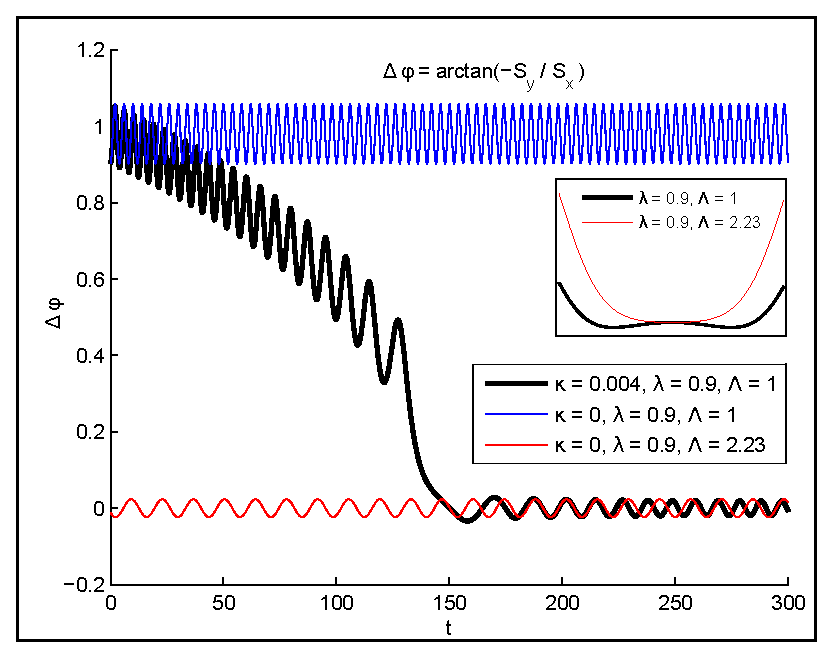
\includegraphics[width=0.7\linewidth]{pic/phase_potential_dissipation.eps}}
\caption{Normalized phase difference as a function of dimensionless time for {\red \dots}.
For red, blue and black curves initial conditions are {\red \dots}, respectively. Inset demonstrates potential behavior for red and blue curves respectively.
\label{pic:phase}}
\end{figure}
%
Adiabaticity condition reads, cf. {\red [ ]}:
%
\begin{equation}
\dfrac{1}{\omega^2(t)} \Big| \dfrac{d \omega}{d t} \Big| \ll 1.
\end{equation}
%
where $\omega(t) = \sqrt{(B - 2\beta(t))(B - 2 \beta(t) + 2 \alpha(t))}$ is small amplitude oscillations slowly depending on time. 

%It allows us to reduce linear system to the harmonic oscillator equaiton with slowly evolving frequency:
%
%\begin{equation}
%\ddot{\phi} + \omega^2(t) \phi = 0,
%\end{equation}
%
The solution of the phase in this case can be given as 
\begin{equation}
\phi(\tau) \approx A / \sqrt{\omega(\tau)} \cos (\omega(\tau) \tau),
\end{equation}
%
where $\tau$ is the time elapsed after the oscillation sets in, and $A$ is an amplitude of oscillations at the moment $\tau = 0$.

Physically, behavior of the system in the presence of dissipation showed in Fig. \ref{pic:phase} establishes non-equilibrium phase transition from quantum (where tunneling is possible) to the classical regime where tunneling is escaped. 

\section{Conclusion \label{sec:conclusion}}

Let us summarize the results obtained. In the paper we examine quantum phase properties for  Josephson junctions created from coupled exciton polariton condensates in the limit of finite temperatures and dissipation. We obtain  various shape of phase potentials depending on the $\Lambda$ and $\lambda$ parameters characterizing condensate junctions. The W-shape potential at finite temperature admits two regimes which are  purely quantum tunneling regime through the barrier or classical regime of thermal activation.   Transition (crossover) between this two limits exhibits universal features of first or second order phase transitions which can be interpreted as phase transition between classical and quantum regimes. It is important that critical temperature of transition depends on some  characteristic temperature  parameter $T_{0}$ (see e.g. (\ref{eq:second_order})) that depends on polariton-polariton interaction (so-called blue shift) $\alpha N$. For experimentally observed values of polariton interaction strength, that implies,say,  $\alpha N=0.3meV$, taken for narrow-band semiconductor samples, the  $T_{0}$ is about $0.6K$ which is less than  typical temperature of condensation, or, temperature of Berezinsky-Kosterlitz-Thouless phase transition considered at thermal equilibrium,cf. {\red [ ]}.  Hence, at large enough temperatures (few tens of Kelvins and more) which are relevant to current experiments with non-equilibrium  exciton polariton condensate junction device operates in classical way. 

The influence of dissipation effects to this picture is evident from our analysis. The thermon lifetime for given  estimations is about $7ps$ that comparable with polariotn lifetime $\tau_{pol}$ in the cavity, cf. {\eqref{eq:lifetime} and [ ]. Thus, the observation of quantum tunneling become possible only within short time intervals when the dissipation cannot essentially affected to the system. Otherwise, after some time interval dissipation leads to crossover in the phase dynamics  and breaking  the evolution of quantum phase in W--potential, see \ref{pic:phase}).    

At the temperatures (or relevant polariton gas densities) sufficiently below the temperature $T_{0}$ of phase transition the exciton polariton condensate junctions are capable for various applications where quantum tunneling effect is crucial. First, it is quantum annealing with exciton polariton condensates that can be enhanced with the help of bosonic stimulation phenomena {\red [ ]}. 

Second, quantum tunneling effect can be explored for design exciton polariton phase qubits, cf. {\red [ ]}. In order, two minima located at the points $A$ and $B$ of $W$-shape quantum phase potential in Fig. \ref{phase_potential}b can be used for initialization of exciton polariton qubit states $\ket{0}$ and $\ket{1}$ similarly to superconductor flux qubits, respectively, {\red cf. [ ]}. However, in our case such qubits much more easier to tailor by external optical or electrical pump {\red [ ]}.  
 
Third, the quantum regime of exciton polariton junctions can be useful for creation of  interferometers with exciton polariton condensates(see e.g. [   ]) for quantum metrology purposes, {\red [ ]}. In particular, we speak here about measurement of the phase shift with high precision accuracy.  It is possible to show that for the Fock regime described by us in the paper the dispersion of the quantum phase approaches to so-callrd Heisenberg limit  ${<(\Delta\phi)^2> \propto \dfrac{1}{N^2}}$ that is 
minimal accessible error for the phase measurement in respect of total particle number.

% Create the reference section using BibTeX:
\bibliography{list}

\end{document}